\documentclass[a4paper,12pt]{article}


\usepackage{graphicx}
\usepackage{tikz}
\usetikzlibrary{positioning, arrows.meta}
\usepackage{amsmath}   
\usepackage{caption}       
\usepackage{xepersian}
\usepackage{setspace}
\usepackage{perpage}
\MakePerPage{footnote}



\renewcommand{\contentsname}{فهرست مطالب\\}
\numberwithin{figure}{subsection}
\settextfont[Extension=.ttf]{IRNazanin}

\begin{document}

\begin{titlepage}

    \centering
   \vspace*{-3cm}
    
    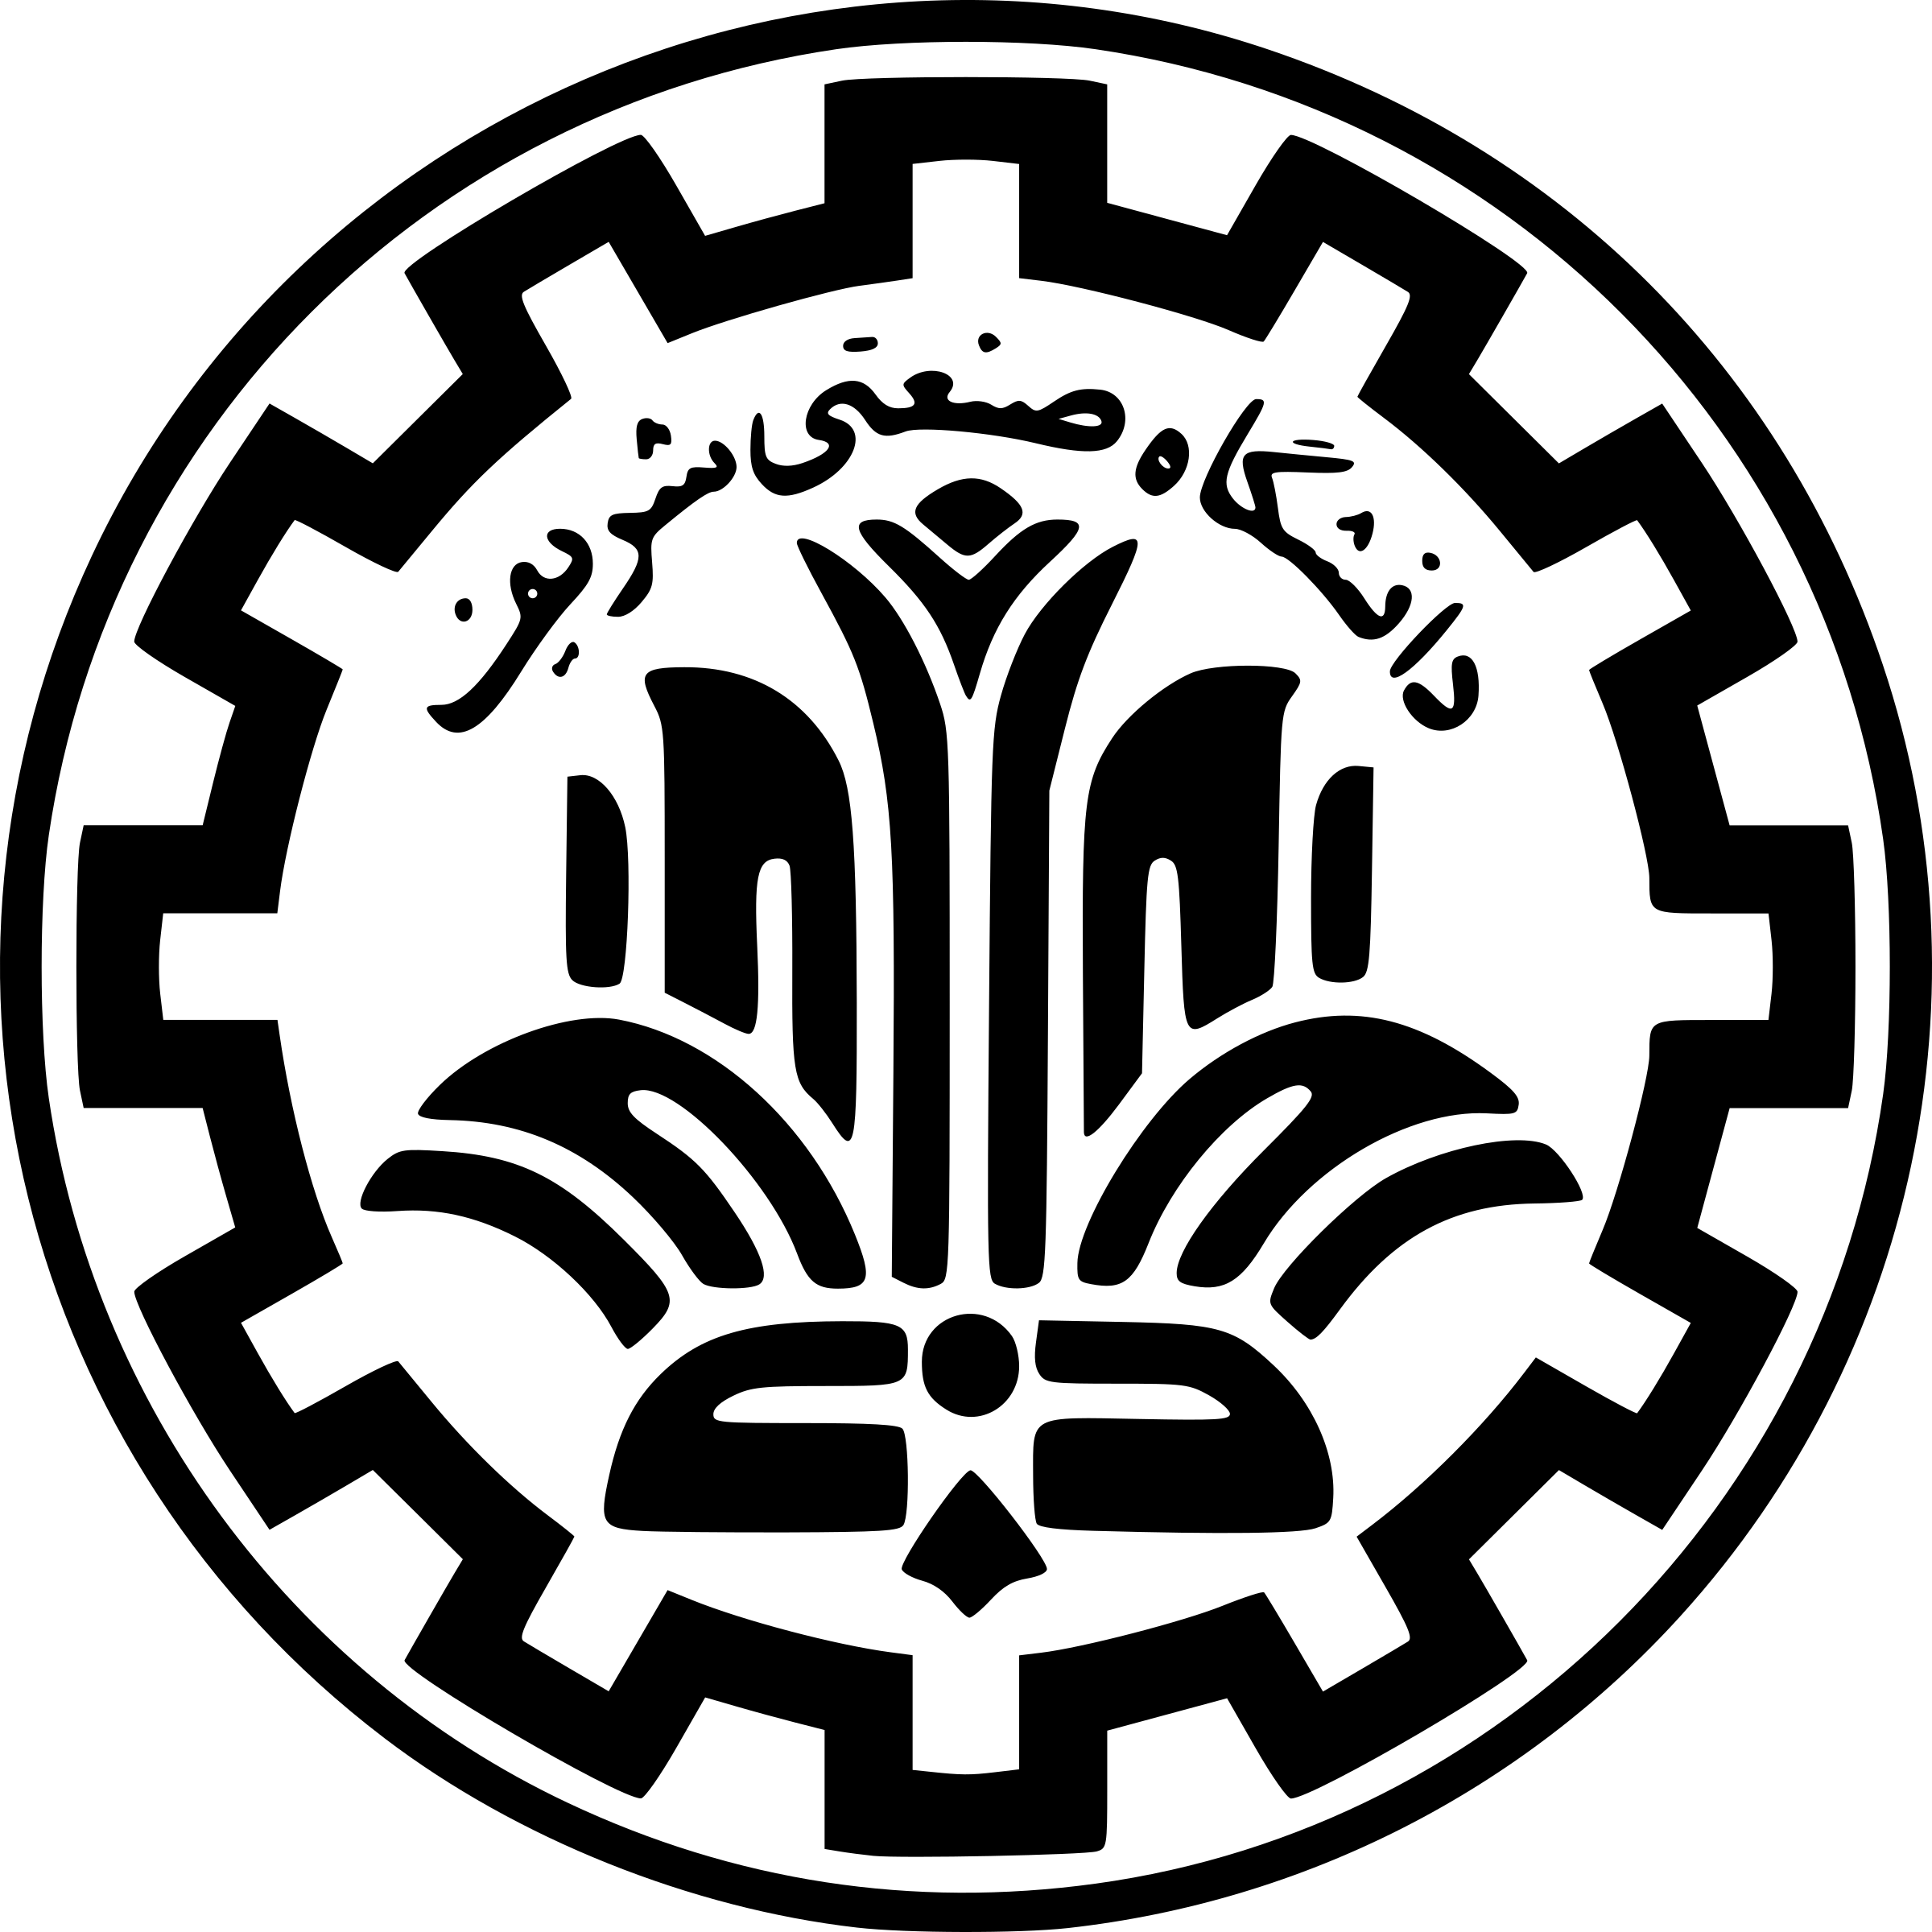
\includegraphics[width=4cm]{images/logo.png} 
    \\[1cm] 
    
    
    {\Large \textbf{گزارش آزمایش}}\\[0.3cm]
    {\Large آزمایشگاه مدار منطقی}\\[1.5cm]
    
    {\LARGE \textbf{آزمایش دوم}}\\[0.5cm]
    {\huge \textbf{شیفت‌رجیستر}}\\[2.5cm]
    
    
    \begin{table}[h]
        \centering
        \large
        

        اعضای گروه:\\
        \vspace{0.5cm}
        \renewcommand{\arraystretch}{1.5} 
        \begin{tabular}{|c|c|}
            \hline
            \textbf{نام و نام خانوادگی} & \textbf{شماره دانشجویی} \\
            \hline
           روناک ابوطالبی & 404105394 \\
            \hline
            حسین مرادی & 404106366 \\
            \hline
        \end{tabular}
    \end{table}
    
    \vspace{2.5cm}
    
    {\large \textbf{تاریخ تحویل: 1405/05/21}}\\[1cm]
    
    {\large \textbf{تابستان 1405}}\\[1cm]
    
    \vfill
    
\end{titlepage}

\newpage
\begin{spacing}{1.5} 
    \tableofcontents 
\end{spacing}


\newpage

\section{مقدمه و تعریف مسئله}
	\leavevmode\par
	\vspace{0.3cm}

\begin{spacing}{1.3} 
در این آزمایش قصد داریم با طراحی و نحوه کارکرد شیفت‌رجیسترها آشنا شویم.
شیفت‌رجیستر نوعی مدار ترتیبی است که از مجموعه‌ای از فلیپ‌فلاپ‌ها(معمولا از نوع \lr{D}) تشکیل شده و برای جابه‌جایی و ذخیره‌سازی موقت اطلاعات باینری به کار می‌رود.

در بخش اول این آزمایش، با استفاده از فلیپ‌فلاپ‌های \lr{D}، یک شیفت‌رجیستر با قابلیت بارگذاری موازی\LTRfootnote{Parallel Load} می‌سازیم. سپس با اعمال تغییرات روی آن، شیفت‌رجیستری با قابلیت شیفت دوطرفه طراحی می‌کنیم.

در بخش دوم با استفاده از تراشه 7495، که یک شیفت‌رجیستر آماده است، مداری برای تشخیص رشته‌های خاص در ورودی طراحی می‌کنیم.

در این آزمایش از نزم‌افزار \lr{Logisim} برای طراحی و تست اولیه مدارها استفاده می‌کنیم و سپس طراحی مدار نهایی را در نرم‌افزار \lr{Proteus} انجام می‌دهیم.
\end{spacing}


\newpage

\section{طراحی و ساخت یک شیفت‌رجیستر}
	\leavevmode\par
	\vspace{0.3cm}
	
	\begin{spacing}{1.3} 
در این بخش از آزمایش قصد داریم با استفاده از فلیپ‌فلاپ‌ها و گیت‌های مورد نیاز یک شیفت‌رجیستر با قابلیت \lr{Parallel Load} و شیفت راست بسازیم. سپس با اعمال ورودی‌های مناسب مقدار اولیه 1010 را در آن ذخیره کنیم. در نهایت با اعمال تغییراتی روی آن، یک شیفت‌رجیستر دوطرفه(بدون قابلیت بارگذاری موازی) بسازیم.
\end{spacing}


\subsection{بررسی و انتخاب روش طراحی}
\leavevmode\par
\vspace{0.2cm}
	
\begin{spacing}{1.3} 
برای ساخت شیفت‌رجیستر، از فلیپ‌فلاپ نوع \lr{D} استفاده می‌کنیم. استفاده از فلیپ‌فلاپ‌های نوع \lr{D} برای ساخت شیفت رجیسترها رایج‌ترین و منطقی‌ترین انتخاب در طراحی مدارهای دیجیتال است. دلیل این موضوع به ساختار و نحوه عملکرد این نوع فلیپ‌فلاپ برمی‌گردد.


ویژگی اصلی این نوع فلیپ‌فلاپ‌ها این است که هر داده‌ای (صفر یا یک) که در پایه ورودی(\lr{D}) قرار داشته باشد را دقیقاً در لبه پالس ساعت(\lr{Clock}) به خروجی(\lr{Q}) منتفل می‌کند.در یک شیفت رجیستر، هدف ما دقیقاً همین است، می‌خواهیم با هر پالس ساعت، داده‌ها یک مرحله به جلو (یا عقب) منتقل شوند. فلیپ‌فلاپ \lr{D} این کار را بدون هیچ پیچیدگی اضافه‌ای انجام می‌دهد.

فلیپ‌فلاپ‌های \lr{D} تنها یک پایه ورودی داده دارند. وقتی می‌خواهیم چندین فلیپ‌فلاپ را پشت سر هم وصل کنیم تا یک شیفت رجیستر بسازیم، کافی است خروجی(\lr{Q}) فلیپ‌فلاپ اول را به ورودی(\lr{D}) فلیپ‌فلاپ دوم وصل کنیم و همین‌طور تا آخر.
اگر بخواهیم از فلیپ‌فلاپ‌های \lr{SR} یا \lr{JK} استفاده کنیم، چون هر کدام دو پایه ورودی دارند، سیم‌کشی روی برد یا داخل تراشه بسیار شلوغ‌تر و پیچیده‌تر می‌شود.
همچنین با استفاده از فلیپ‌فلاپ نوع \lr{D} نیاز نیست نگران حالات غیرمجاز(که در فلیپ‌فلاپ نوع \lr{SR} وجود دارد) باشیم.

برای تعیین عمکرد شیفت‌‍رجیستر با ورودی کنترلی \lr{$Mode$} و جابه‌حای شدن بین حالت های «ثبت ورودی موازی» و «شیفت راست» یا «شیفت راست» و «شیفت چپ»، ابتدا \lr{$Mode$} یا \lr{$\overline{Mode}$} را با ورودی مربوط به هرکدام \lr{AND} می‌کنیم و سپس تمام حالات ممکن ورودی هر فلیپ‌فلاپ را با هم \lr{OR} کرده و به ورودی فلیپ‌فلاپ می‌فرستیم.
\end{spacing}

\subsection{بلوک‌دیاگرام طرح پیشنهادی اولیه}
\leavevmode\par
\vspace{0.2cm}

\begin{center}
\begin{tikzpicture}[
    node distance=1cm and 0.8cm,
    basebox/.style={
        rectangle, draw=black, thick, rounded corners=1mm,
        minimum height=1.2cm, minimum width=1.8cm, align=center
    },
    greenbox/.style={basebox, fill=green!10},
    bluebox/.style={basebox, fill=blue!10},
    arrow/.style={-Latex, thick}
]

    \node[greenbox] (input) {ورودی‌ها \\ \lr{A..D, $S_{in}$}};
    \node[bluebox, right=of input] (mode) { \lr{Mode}};
    \node[bluebox, above=of mode] (right-shift) {\lr{Right Shift}};
    \node[bluebox, right=of right-shift] (sin) {\lr{$S_{in} \to FF_A$}};
    \node[bluebox, below=of mode] (pin) {\lr{Parallel Load}};
    
   
    \node[greenbox, right=of sin] (out) {خروجی \\ \lr{Q$_A$..Q$_D$}};

    \draw[arrow] (input) -- (mode);
    \draw[arrow] (mode) -- (right-shift)node[midway, left, font=\small] {$0$};
    \draw[arrow] (mode) -- (pin)node[midway, left, font=\small] {$1$};
    \draw[arrow] (right-shift) -- (sin);
    \draw[arrow] (sin) -- (out);
    \draw[arrow] (pin) -- (out);
   

\end{tikzpicture}
\captionof{figure}{بلوک‌دیاگرام شیفت‌رجیستر با ورودی موازی/سریالی و شیفت راست }
\label{fig:blockdiagram1}

\vspace{0.4cm}

\begin{tikzpicture}[
    node distance=1cm and 0.8cm,
    basebox/.style={
        rectangle, draw=black, thick, rounded corners=1mm,
        minimum height=1.2cm, minimum width=1.8cm, align=center
    },
    greenbox/.style={basebox, fill=green!10},
    bluebox/.style={basebox, fill=blue!10},
    arrow/.style={-Latex, thick}
]

	\node[greenbox] (input) {ورودی‌ها \\ \lr{A..D, $S_{in}$}};
    \node[bluebox, right=of input] (mode) { \lr{Mode}};
    \node[bluebox, above=of mode] (right-shift) {\lr{Right Shift}};
    \node[bluebox, below=of mode] (left-shift) {\lr{Left Shift}};
    \node[greenbox, right=of mode] (out) {خروجی \\ \lr{Q$_A$..Q$_D$}};
    
    \draw[arrow] (input) -- (mode);
    \draw[arrow] (mode) -- (right-shift)node[midway, left, font=\small] {$0$};
    \draw[arrow] (mode) -- (left-shift)node[midway, left, font=\small] {$1$};
    \draw[arrow] (right-shift) -- (out);
    \draw[arrow] (left-shift) -- (out);

\end{tikzpicture}
\captionof{figure}{بلوک‌دیاگرام شیفت‌رجیستر با شیفت دوطرفه }
\label{fig:blockdiagram2}
\end{center}

\subsection{روند پیاده‌سازی}
\leavevmode\par
\vspace{0.2cm}

\begin{spacing}{1.3} 
در حالت کلی، شیفت‌رجیستر از بستن متوالی فلیپ‌فلاپ‌ها به هم ساخته می‌شود. در ساده ترین نوع شیفت‌رجیستر، خروجی(\lr{Q}) هر فلیپ‌فلاپ به ورودی(\lr{D}) فلیپ‌فلاپ بعدی متصل می‌شود. در این آزمایش، چون نیاز به قابلیت \lr{Parralel Load} و همچنین توانایی کنترل عملکرد مدار با استفاده از ورودی \lr{$Mode$} داریم، ورودی فلیپ‌فلاپ ها را با استفاده از توابع ساده‌ای که با گیت های \lr{AND}، \lr{OR} و \lr{NOT} ساخته می‌شوند می‌سازیم.
\end{spacing}

\subsection{شماتیک طرح اولیه}
\leavevmode\par
\vspace{0.2cm}

\begin{spacing}{1.3} 
در این‌جا طرح اولیه هر بخش را در نرم‌افزار \lr{Proteus} پیاده‌سازی کردیم.
\end{spacing}

\begin{center}
    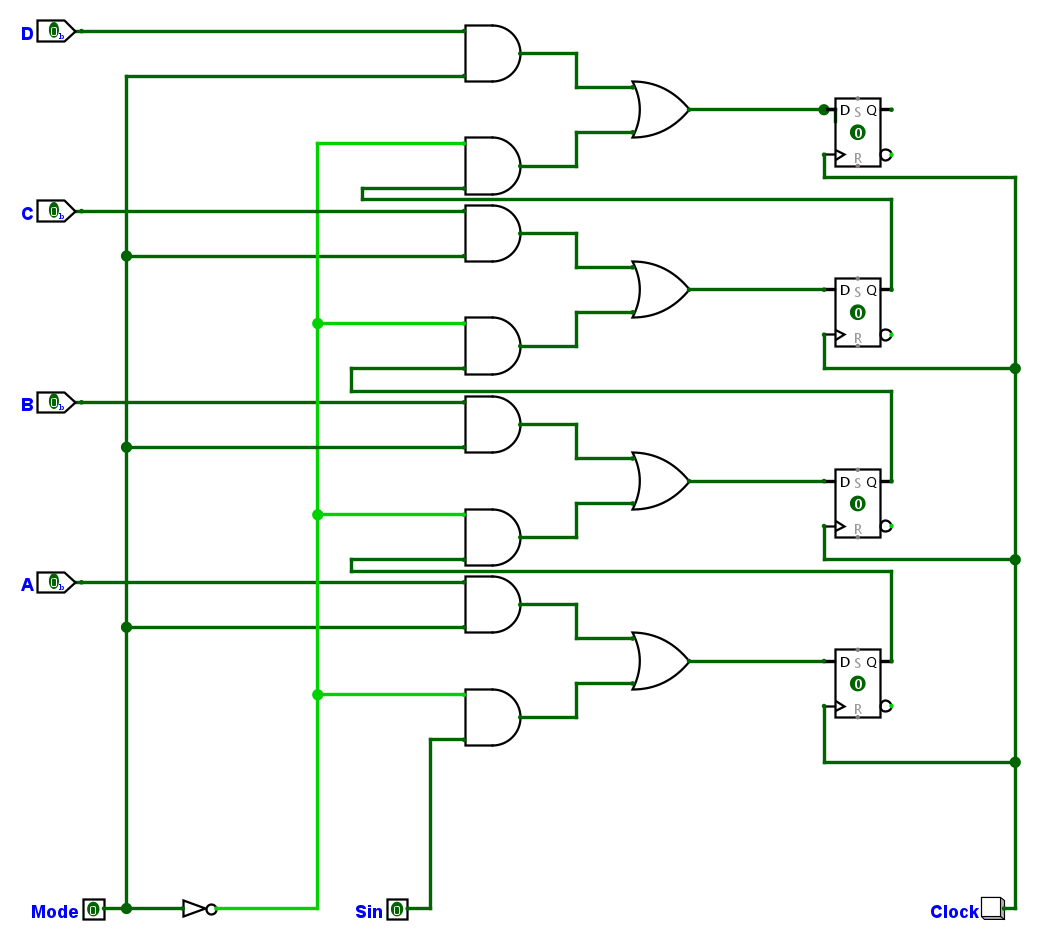
\includegraphics[width=1\textwidth]{images/1/log11.png}
    \captionof{figure}{شیفت‌رجیستر با قابلیت شیفت راست و ورودی موازی/سریالی}
    \label{fig:log11}
\end{center}

\begin{center}
    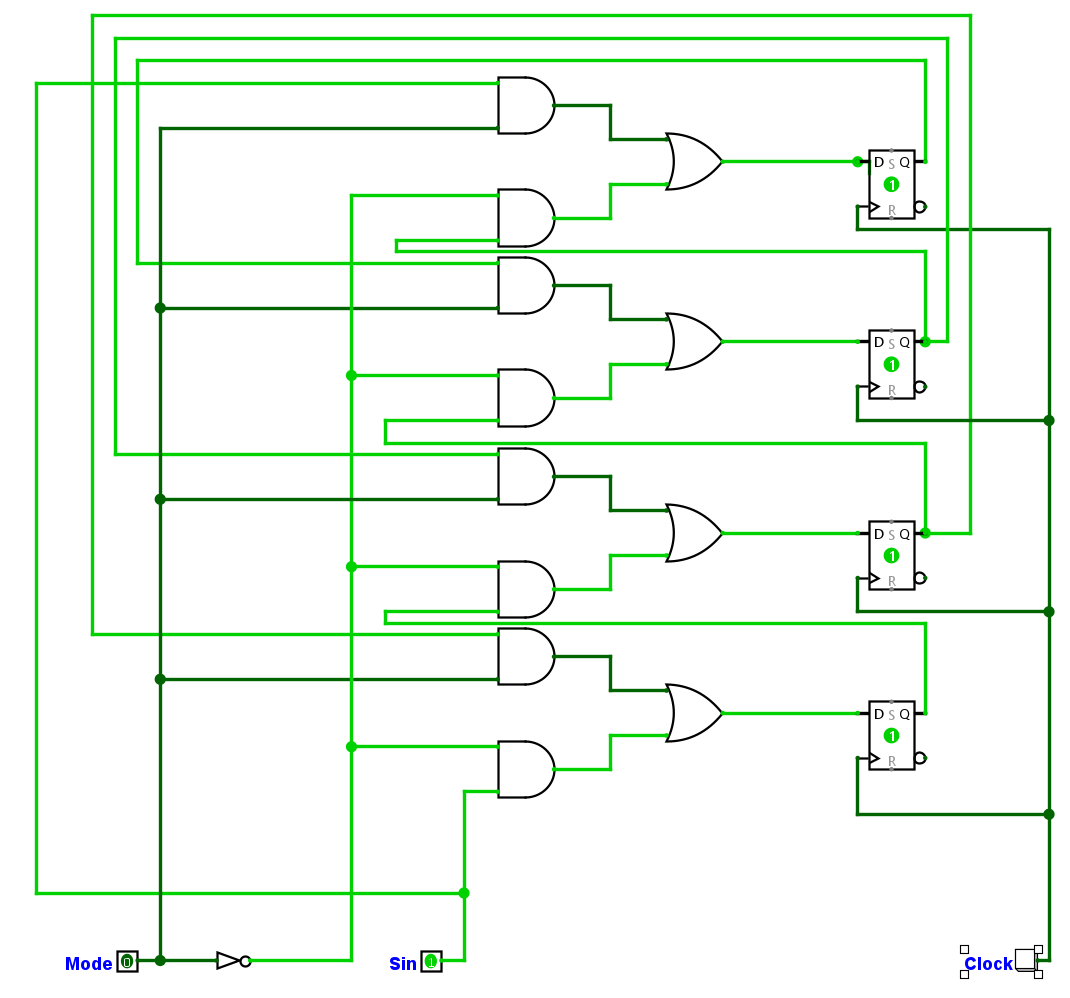
\includegraphics[width=1\textwidth]{images/1/log12.png}
    \captionof{figure}{شیفت‌رجیستر با قابلیت شیفت دوطرفه }
    \label{fig:log12}
\end{center}


\subsection{شماتیک نهایی مدار}
\leavevmode\par
\vspace{0.2cm}

\begin{spacing}{1.3} 
مدار نهایی، تفاوت قابل توجهی با شماتیک اولیه ندارد. در اینجا از نرم‌افزار \lr{Proteus} استفاده کرده‌ایم.
\end{spacing}

\begin{center}
    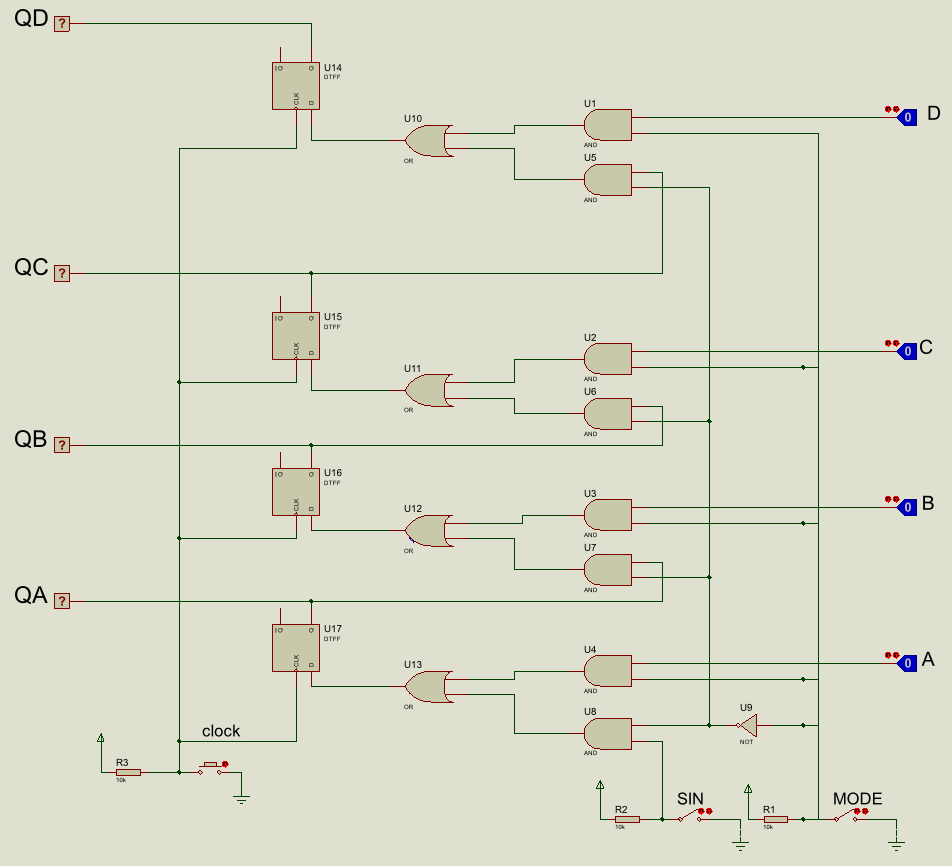
\includegraphics[width=1\textwidth]{images/1/pr11.png}
    \captionof{figure}{شیفت‌رجیستر با قابلیت شیفت راست و ورودی موازی/سریالی}
    \label{fig:pr11}
\end{center}

\begin{center}
    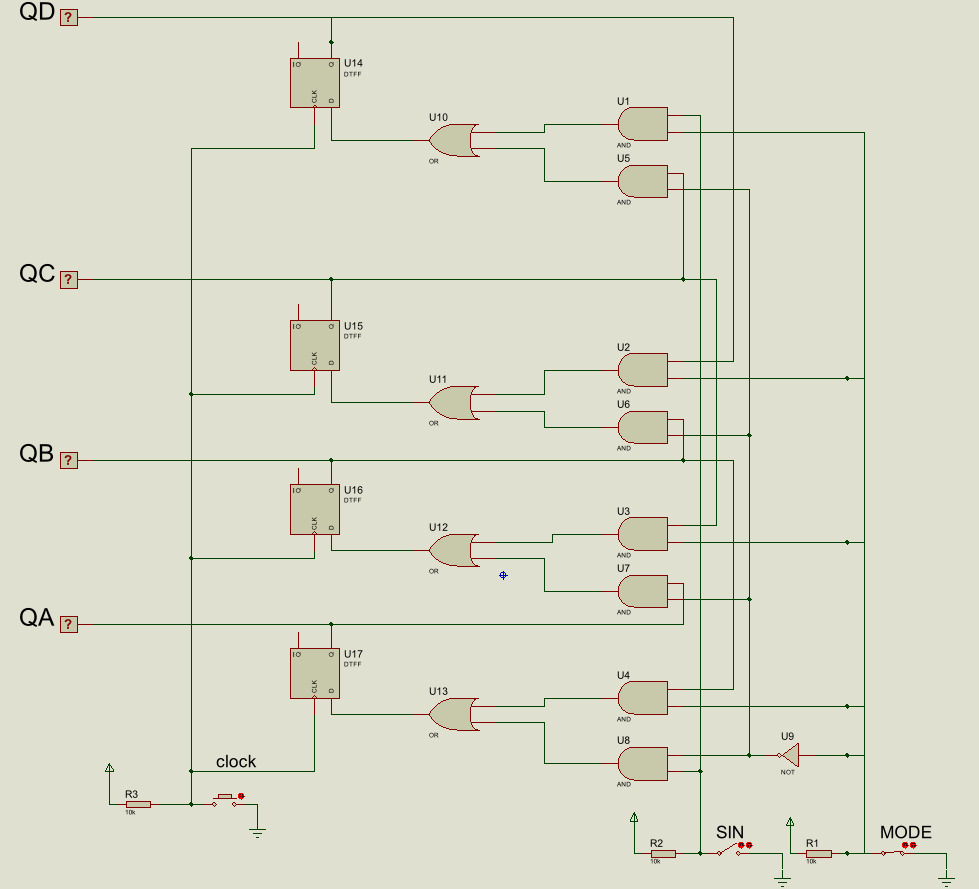
\includegraphics[width=1\textwidth]{images/1/pr12.png}
    \captionof{figure}{شیفت‌رجیستر با قابلیت شیفت دوطرفه }
    \label{fig:pr12}
\end{center}

\subsection{بررسی \lr{Test Case} ها}
\leavevmode\par
\vspace{0.3cm}

\subsection*{مدار داری قابلیت بارگذاری موازی}
\leavevmode\par
\vspace{0.2cm}

\begin{spacing}{1.3}
ابتدا قابلیت بارگذاری موازی را با مقدار اولیه داده شده در صورت سوال(\lr{1010}) تست می‌کنیم. سپس شیفت راست را امتحان می‌کنیم.
\end{spacing}

\begin{center}
    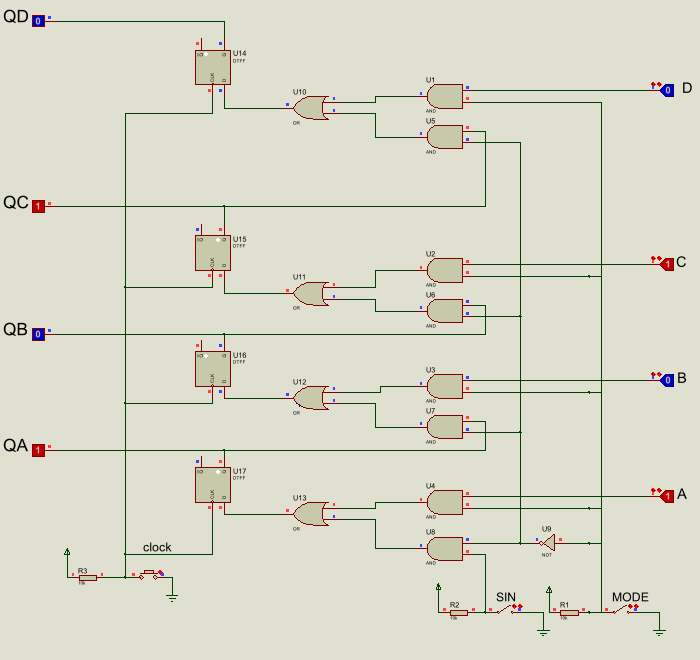
\includegraphics[width=1\textwidth]{images/1/plt.png}
    \captionof{figure}{تست بارگذاری موازی\newline
    \begin{latin}
    $ABCD = 1010 , Mode = 1 \to Q_AQ_BQ_CQ_D = 1010$
    \end{latin}
    }
    \label{fig:plt}
\end{center}

\begin{center}
    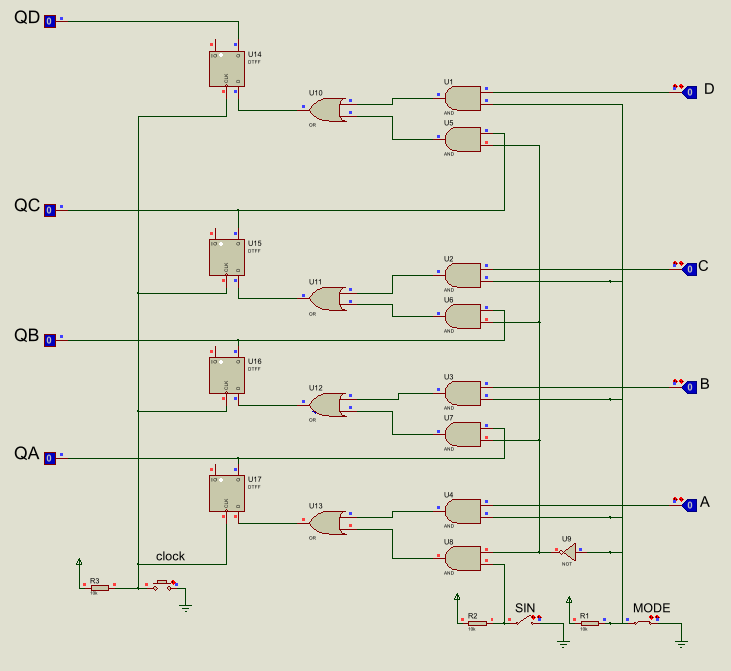
\includegraphics[width=1\textwidth]{images/1/rst1.png}
    \captionof{figure}{تست شیفت راست در \lr{$T_1$}}
    \label{fig:rst1}
\end{center}

\begin{center}
    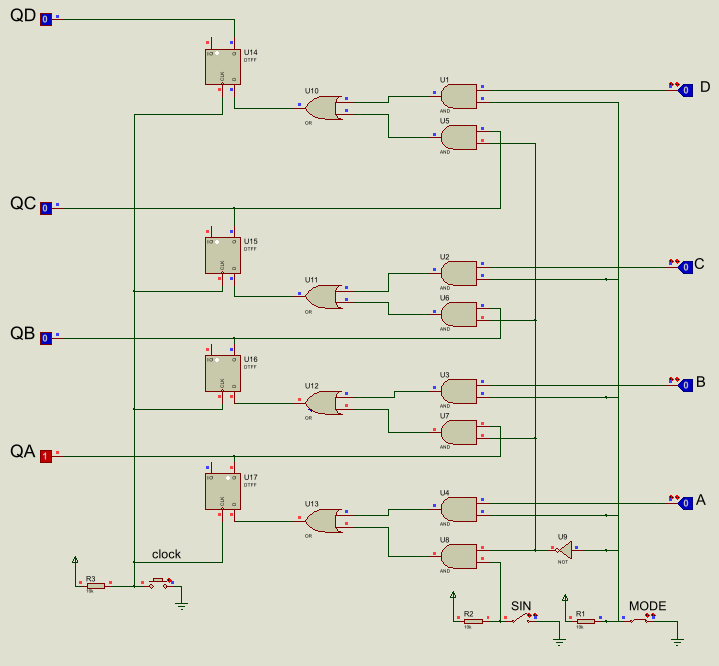
\includegraphics[width=1\textwidth]{images/1/rst2.png}
    \captionof{figure}{تست شیفت راست در \lr{$T_2$}}
    \label{fig:rst2}
\end{center}

\begin{center}
    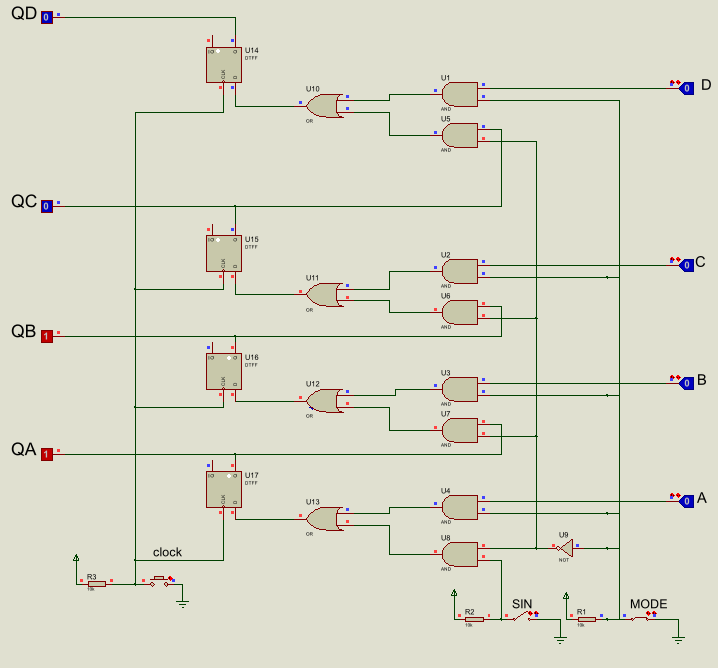
\includegraphics[width=1\textwidth]{images/1/rst3.png}
    \captionof{figure}{تست شیفت راست در \lr{$T_3$}}
    \label{fig:rst3}
\end{center}

\begin{center}
    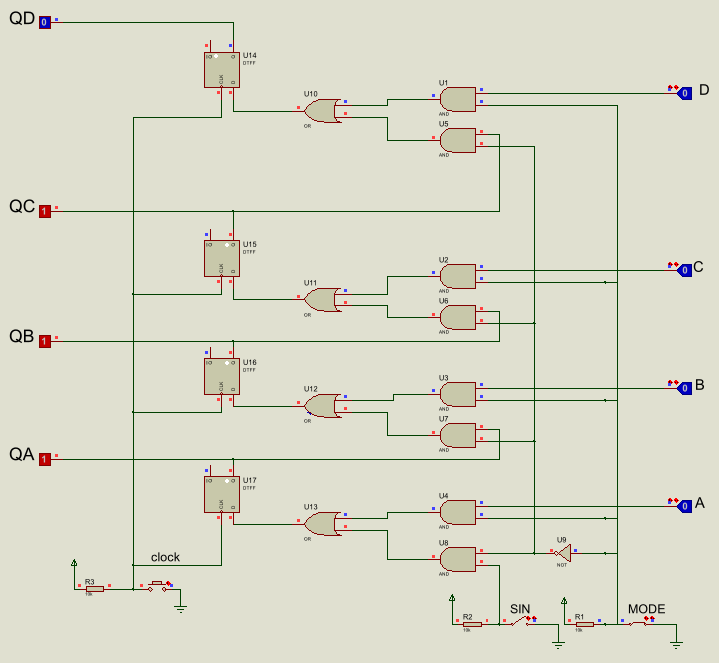
\includegraphics[width=1\textwidth]{images/1/rst4.png}
    \captionof{figure}{تست شیفت راست در \lr{$T_4$}}
    \label{fig:rst4}
\end{center}

\begin{spacing}{1.3} 
همانطور که مشاهده شد، به ازای \lr{$S_{in} = 1$} برای چهار کلاک، شیفت راست به درستی انجام شد.
\end{spacing}


\begin{latin}
$0000 \to 1000 \to 1100 \to 1110$
\end{latin}

\newpage

\subsection*{مدار داری قابلیت شیفت دوطرفه}
\leavevmode\par
\vspace{0.2cm}

\begin{center}
    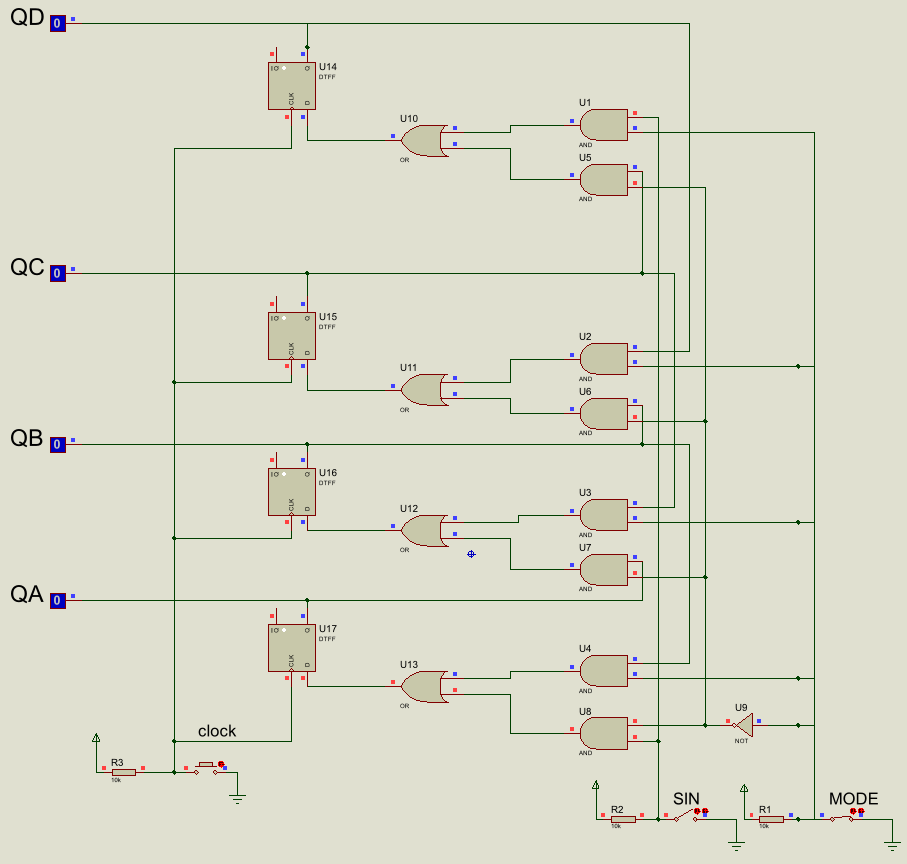
\includegraphics[width=1\textwidth]{images/1/bst1.png}
    \captionof{figure}{حالت اولیه مدار در \lr{$T_1$}}
    \label{fig:bst1}
\end{center}

\begin{center}
    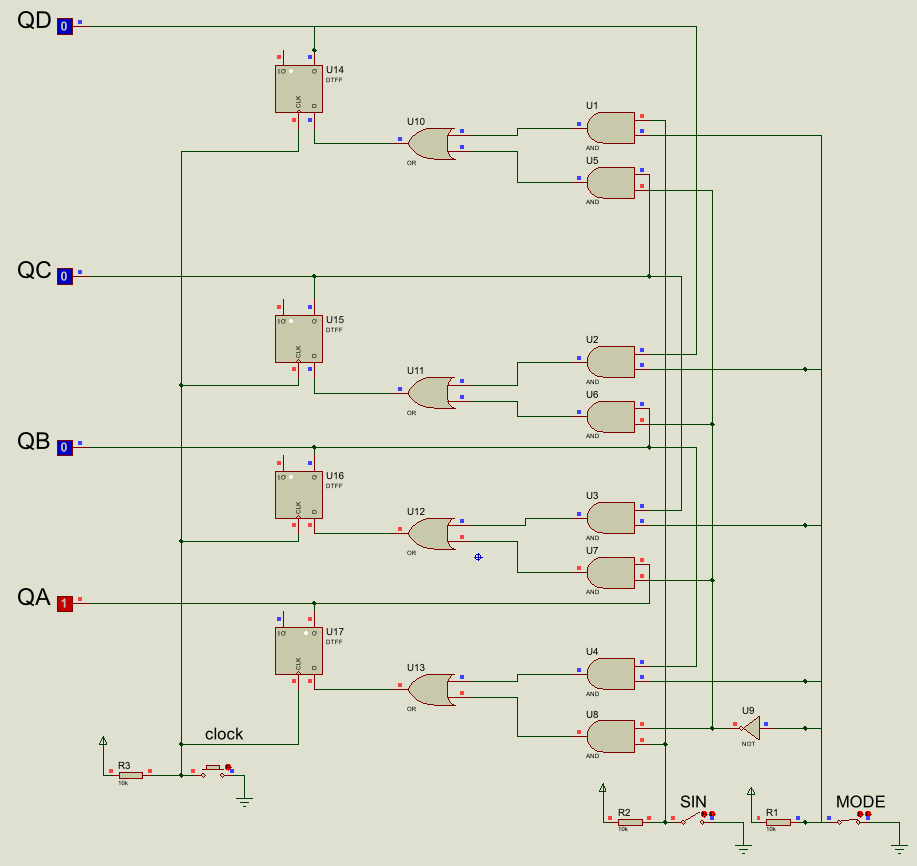
\includegraphics[width=1\textwidth]{images/1/bst2.png}
    \captionof{figure}{پس از یک شیفت راست با \lr{$S_{in} = 1$} در \lr{$T_2$}}
    \label{fig:bst2}
\end{center}

\begin{center}
    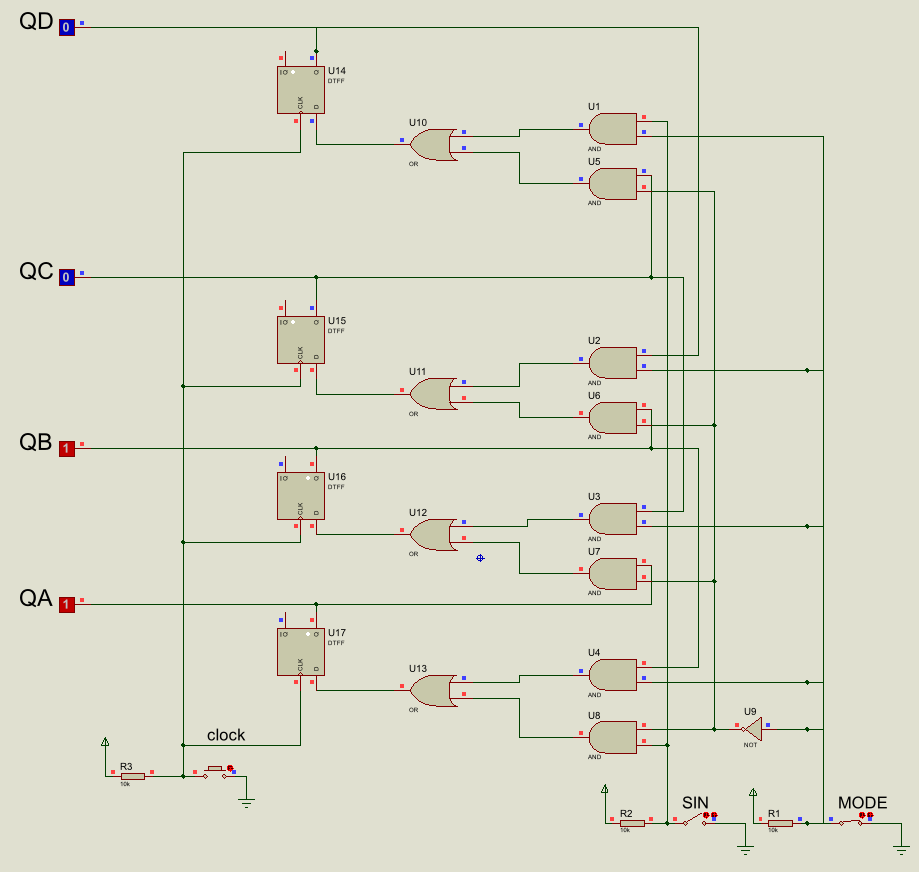
\includegraphics[width=1\textwidth]{images/1/bst3.png}
    \captionof{figure}{پس از یک شیفت راست دیگر با \lr{$S_{in} = 1$} در \lr{$T_3$}}
    \label{fig:bst3}
\end{center}

\begin{center}
    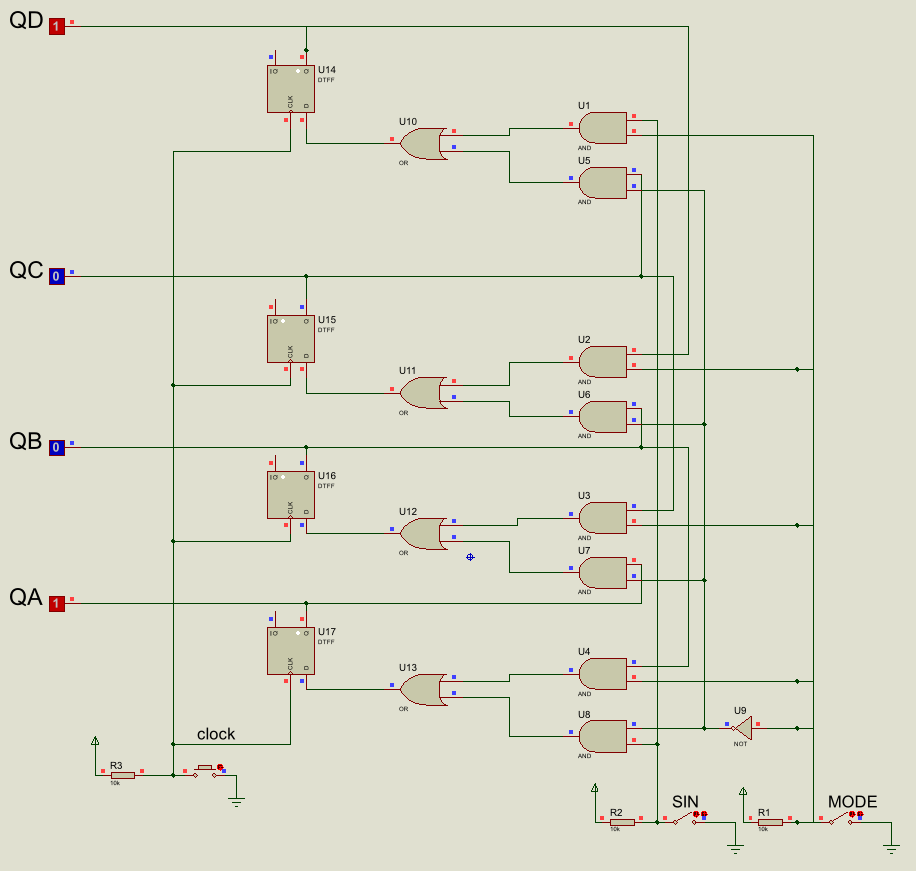
\includegraphics[width=1\textwidth]{images/1/bst4.png}
    \captionof{figure}{پس از یک شیفت چپ با \lr{$S_{in} = 1$} در \lr{$T_4$}}
    \label{fig:bst4}
\end{center}

\begin{center}
    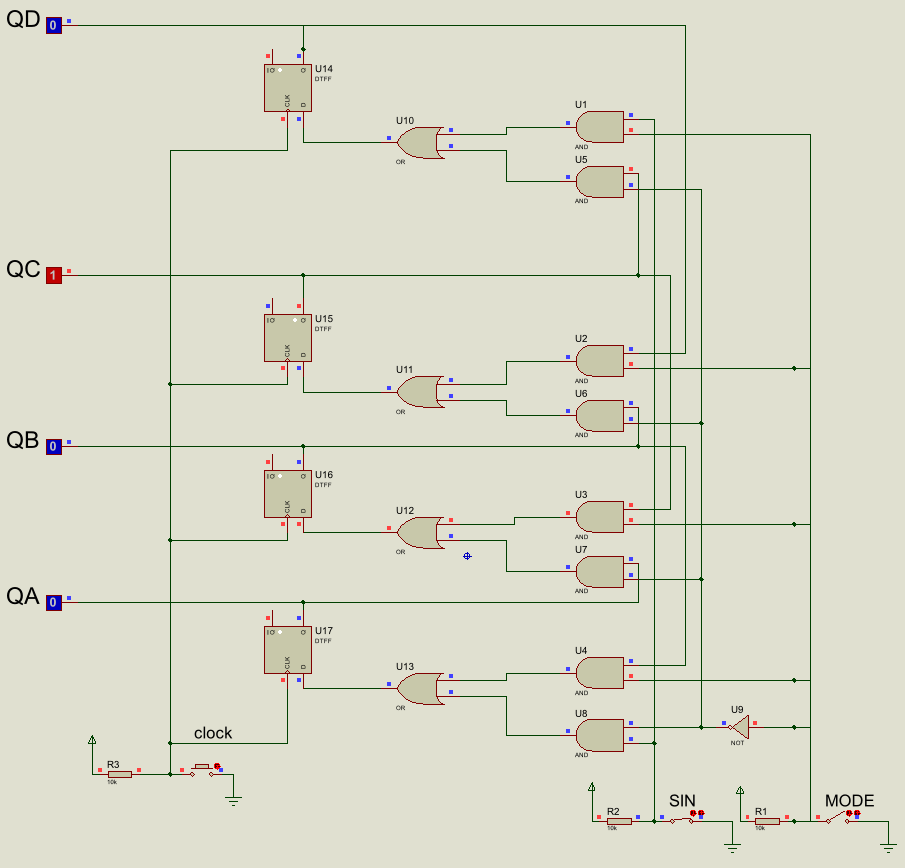
\includegraphics[width=1\textwidth]{images/1/bst5.png}
    \captionof{figure}{پس از یک شیفت چپ با \lr{$S_{in} = 0$} در \lr{$T_5$}}
    \label{fig:bst5}
\end{center}



\begin{spacing}{1.3} 
در این مدار نیز نتیجه تست‌ با انتظارات ما مطابقت دارد.
\end{spacing}

\begin{latin}
$$0000 \xrightarrow{S_{in} = 1, \text{R-Shift}} 1000 \xrightarrow{S_{in} = 1, \text{R-Shift}} 1100 \xrightarrow{S_{in} = 1, \text{L-Shift}} 1001 \xrightarrow{S_{in} = 0, \text{L-Shift}} 0010$$
\end{latin}

\newpage


\section{استفاده از شیفت‌رجیستر آماده}
	\leavevmode\par
	\vspace{0.3cm}
	\begin{spacing}{1.3} 
در این قسمت از تراشه 7495 استفاده می‌کنیم و در نهایت مداری طراحی می‌کنیم که بتواند رشته‌های ورودی خاص را تشخیص دهد.
\end{spacing}

\subsection{بررسی و انتخاب روش طراحی}
\leavevmode\par
\vspace{0.2cm}

\begin{spacing}{1.3} 
ابتدا باید با تراشه 7495 آشنا شویم. این تراشه 14 پایه دارد که پایه‌های 7 و 14 به ترتیب \lr{GND} و \lr{VCC} هستند. پایه‌ 1 ورودی سریالی\LTRfootnote{Serial Input} و پایه های 2 تا 5 ورودی‌های موازی\LTRfootnote{Parallel Inputs}، پایه های 10 تا 13 خروجی‌ها و پایه 6 ورودی کنترلی(\lr{Mode}) می‌باشد. پایه های 8 و 9 پایه‌های کلاک برای حالت‌های بارگذاری موازی و شیفت راست هستند.
برای تشخیص رشته‌های ورودی مورد نظر- که در اینجا \lr{0001, 0010, 1110, 1101} هستند- از گیت های اصافه استفاده می‌کنیم. برای ساختن تابع خروجی، می‌توان مانند هر تابع دیگری از جدول کارنو استفاده کرد.
\end{spacing}

\subsection{بلوک‌دیاگرام طرح پیشنهادی اولیه}
\leavevmode\par
\vspace{0.2cm}

\begin{center}
\begin{tikzpicture}[
    node distance=1cm and 0.8cm,
    basebox/.style={
        rectangle, draw=black, thick, rounded corners=1mm,
        minimum height=1.2cm, minimum width=1.8cm, align=center
    },
    greenbox/.style={basebox, fill=green!10},
    bluebox/.style={basebox, fill=blue!10},
    arrow/.style={-Latex, thick}
]

    \node[greenbox] (input) {ورودی‌ها \\ \lr{A..D, $S_{in}$}};
    \node[bluebox, right=of input] (mode) { \lr{Mode}};
    \node[bluebox, above=of mode] (right-shift) {\lr{Right Shift}};
    \node[bluebox, below=of mode] (pin) {\lr{Parallel Load}};
    
   
    \node[greenbox, right=of right-shift] (out) {خروجی \\ \lr{Q$_A$..Q$_D$}};

    \draw[arrow] (input) -- (mode);
    \draw[arrow] (mode) -- (right-shift)node[midway, left, font=\small] {$0$};
    \draw[arrow] (mode) -- (pin)node[midway, left, font=\small] {$1$};
    \draw[arrow] (right-shift) -- (out);
    \draw[arrow] (pin) -- (out);
   

\end{tikzpicture}
\captionof{figure}{بلوک‌دیاگرام شیفت‌رجیستر آماده تراشه 7495 }
\label{fig:blockdiagram3}
\end{center}

\subsection{روند پیاده‌سازی}
\leavevmode\par
\vspace{0.2cm}

\begin{spacing}{1.3} 
ابتدا پایه‌های تراشه را متصل میکنیم. سپس، با استفاده از جدول کارنو، یا هر روش ساده‌سازی، متوجه می‌شویم اگر رشته ذخیره شده در شیفت‌رجیستر \lr{$Q_3Q_2Q_1Q_0$} باشد، تابع زیر در صورتی که یکی از رشته‌های مورد نظر در ورودی ظاهر شده باشد خروجی یک می‌دهد.
\end{spacing}

$$\overline{Q_3}.\overline{Q_2}.\overline{Q_2}.Q_0 + \overline{Q_3}.\overline{Q_2}. Q_1 . \overline{Q_0} + Q_3 . Q_2 . Q_1 . \overline{Q_0} + Q_3 . Q_2 . \overline{Q_1} . Q_0 $$

\begin{spacing}{1.3} 
البته این تابع را می‌توان به شکل‌های دیگر و با استفاده از گیت های دیگر نیز بازنویسی کرد. برای مثال اگر از گیت‌های \lr{XOR} استفاده کینم مدار کمی ساده تر می‌شود:
\end{spacing}

$$(\overline{Q_3 \oplus Q_2}) (Q_1 \oplus Q_0)$$

\subsection{شماتیک طرح اولیه}
\leavevmode\par
\vspace{0.2cm}

\begin{spacing}{1.3} 
شماتیک اولیه مدار را در نرم‌افزار \lr{Logisim} رسم کردیم. در اینجا به دلیل محدودیت قطعات موجود در این نرم‌افزار، از تراشه مشابه استفاده کردیم.
\end{spacing}

\begin{center}
    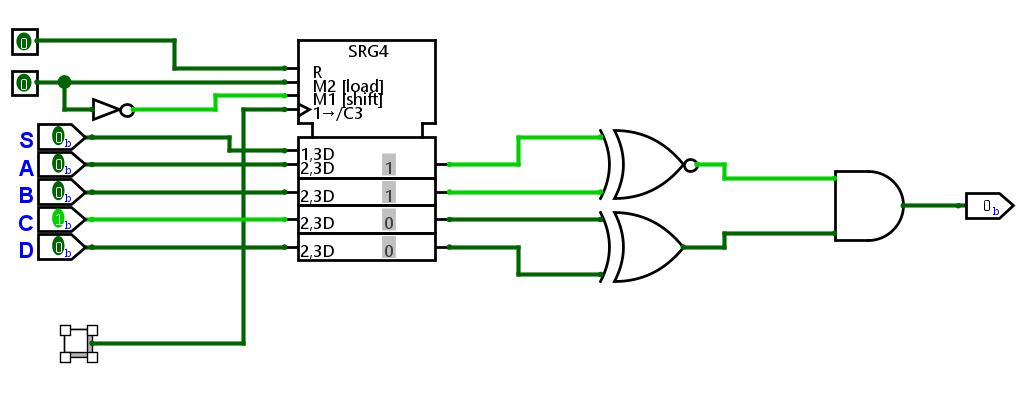
\includegraphics[width=1\textwidth]{images/2/log21.png}
    \captionof{figure}{}
    \label{fig:log21}
\end{center}

\subsection{شماتیک نهایی مدار}
\leavevmode\par
\vspace{0.2cm}

\begin{spacing}{1.3} 
سپس در نرم‌افزار \lr{Proteus} ابتدا تراشه 7495 را می‌بندیم و سپس مدار تشخیص‌دهنده رشته‌های ورودی را اضافه می‌کنیم.
\end{spacing}

\begin{center}
    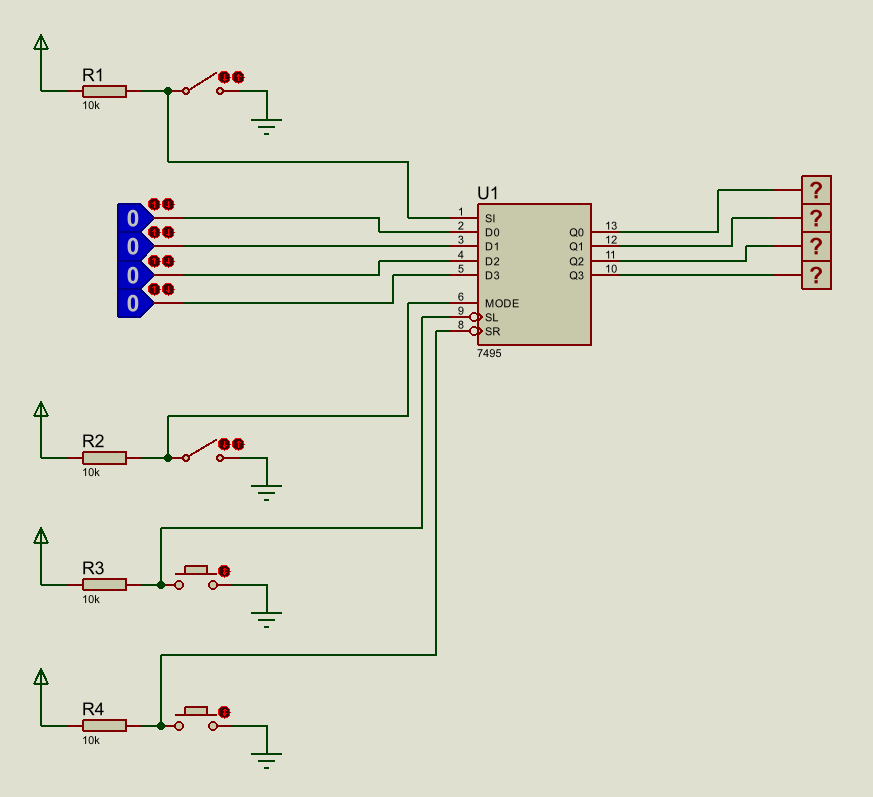
\includegraphics[width=1\textwidth]{images/2/pr21.png}
    \captionof{figure}{تراشه 7495}
    \label{fig:pr21}
\end{center}

\begin{center}
    \begin{minipage}{\textwidth}
        \centering
        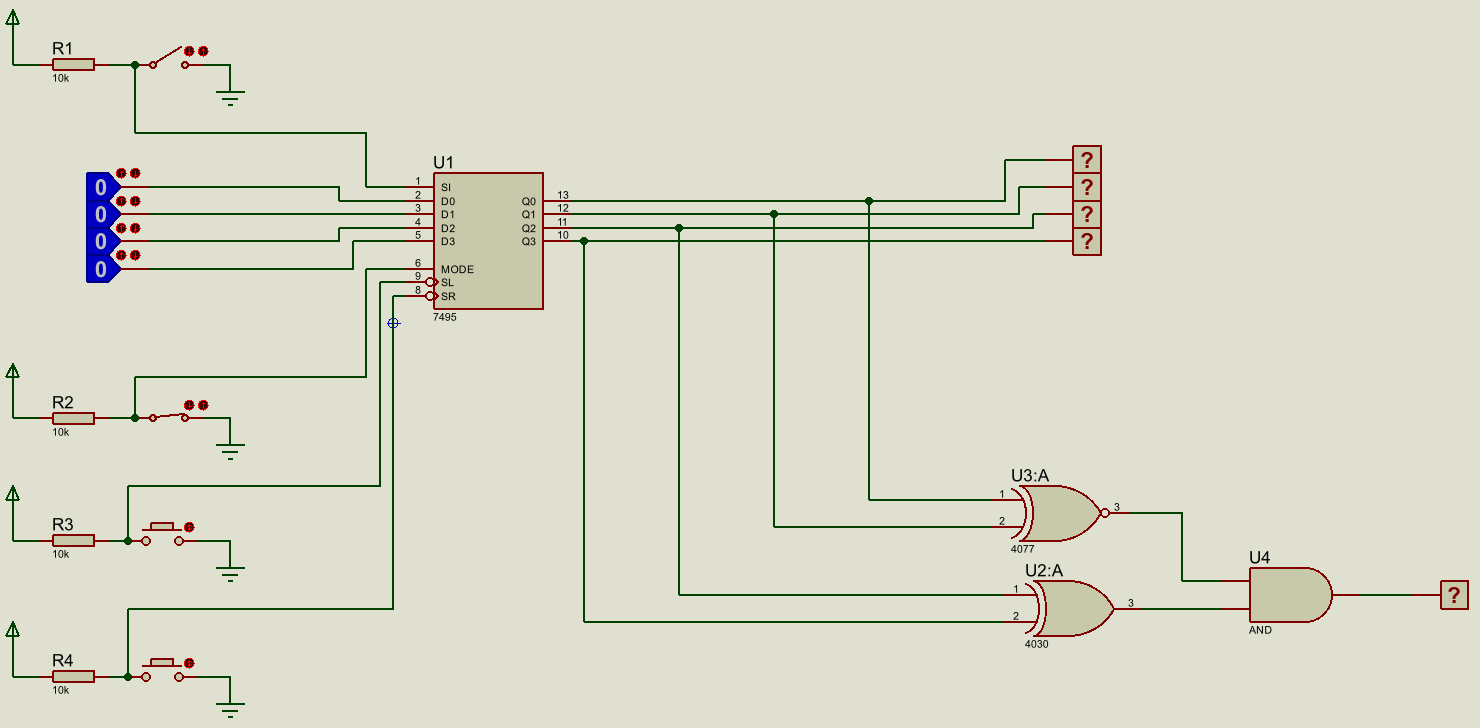
\includegraphics[width=\textwidth]{images/2/pr22.png}
        \captionof{figure}{مدار تشخیص‌دهنده رشته‌های ورودی}
        \label{fig:pr22}
    \end{minipage}
\end{center}

\subsection{بررسی \lr{Test Case} ها}
\leavevmode\par
\vspace{0.3cm}

\begin{center}
    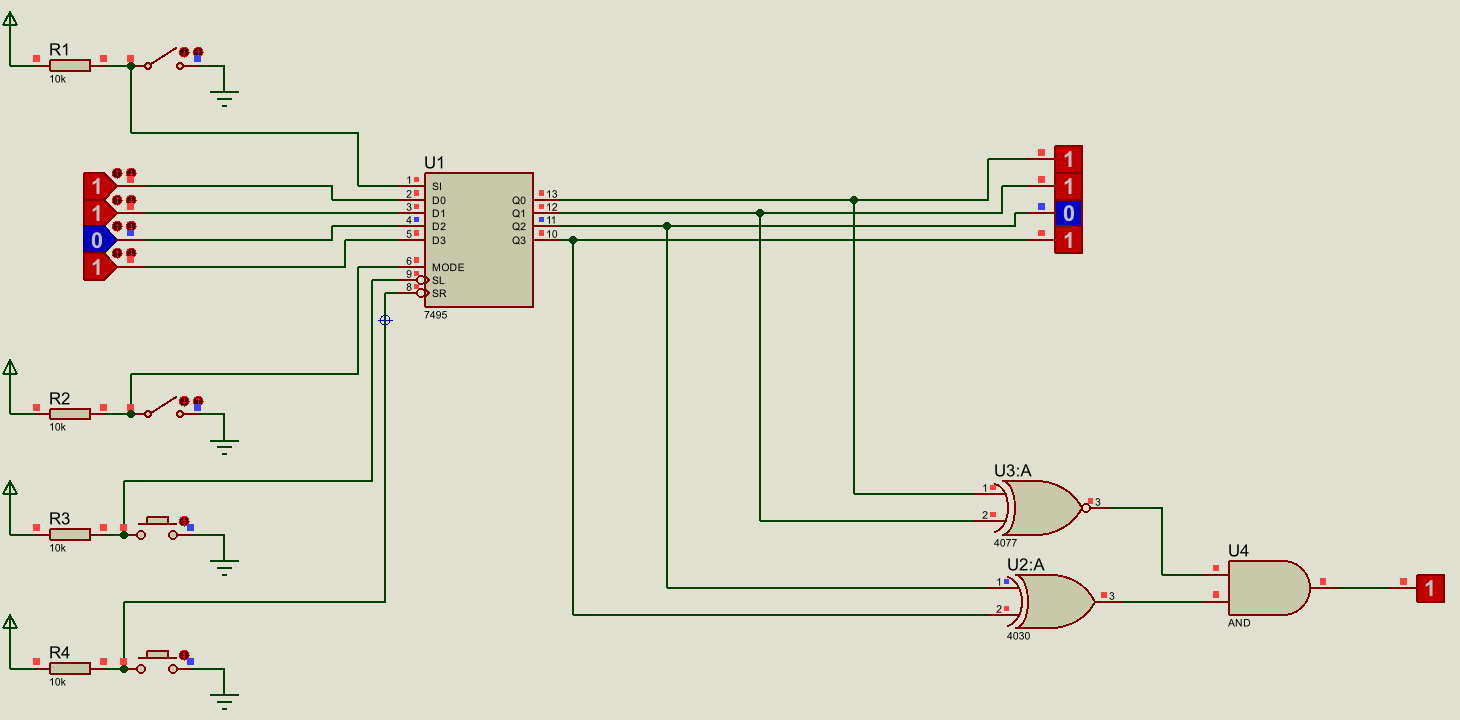
\includegraphics[width=1\textwidth]{images/2/t1.png}
    \captionof{figure}{بررسی بارگذاری موازی و تشخیص رشته وروری}
    \label{fig:t1}
\end{center}

\begin{center}
    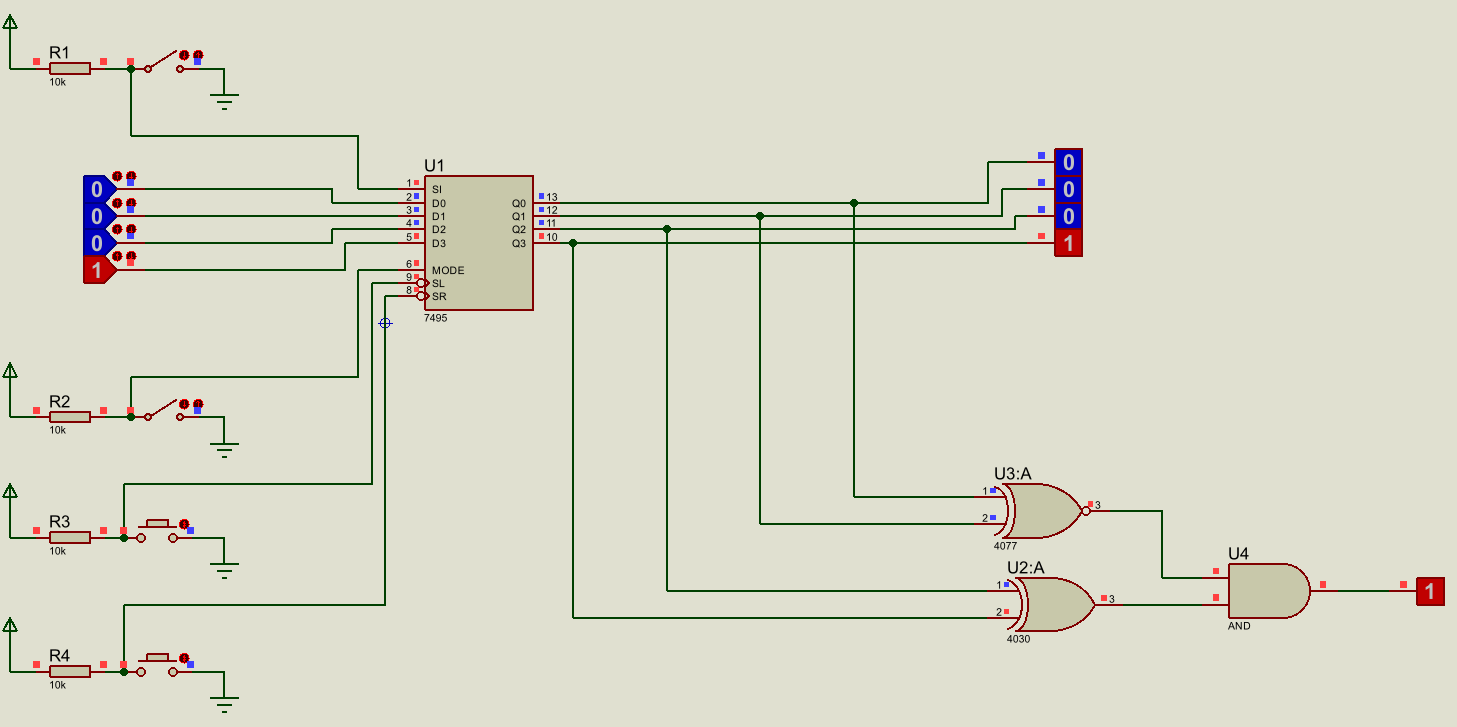
\includegraphics[width=1\textwidth]{images/2/t2.png}
    \captionof{figure}{بررسی بارگذاری موازی و تشخیص رشته وروری}
    \label{fig:t2}
\end{center}

\begin{center}
    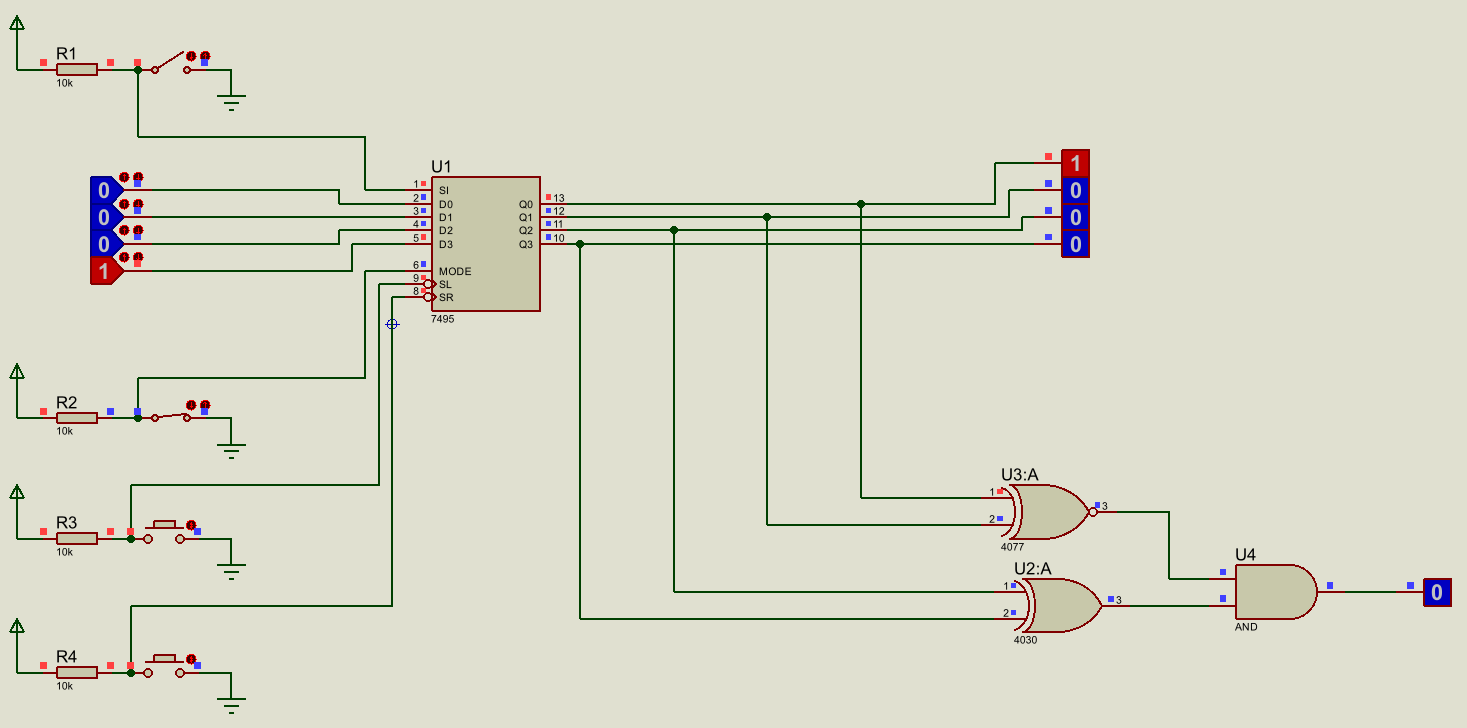
\includegraphics[width=1\textwidth]{images/2/t3.png}
    \captionof{figure}{یک شیفت راست با \lr{$S_{in} = 1$} نسبت به تصویر قبل}
    \label{fig:t3}
\end{center}

\begin{center}
    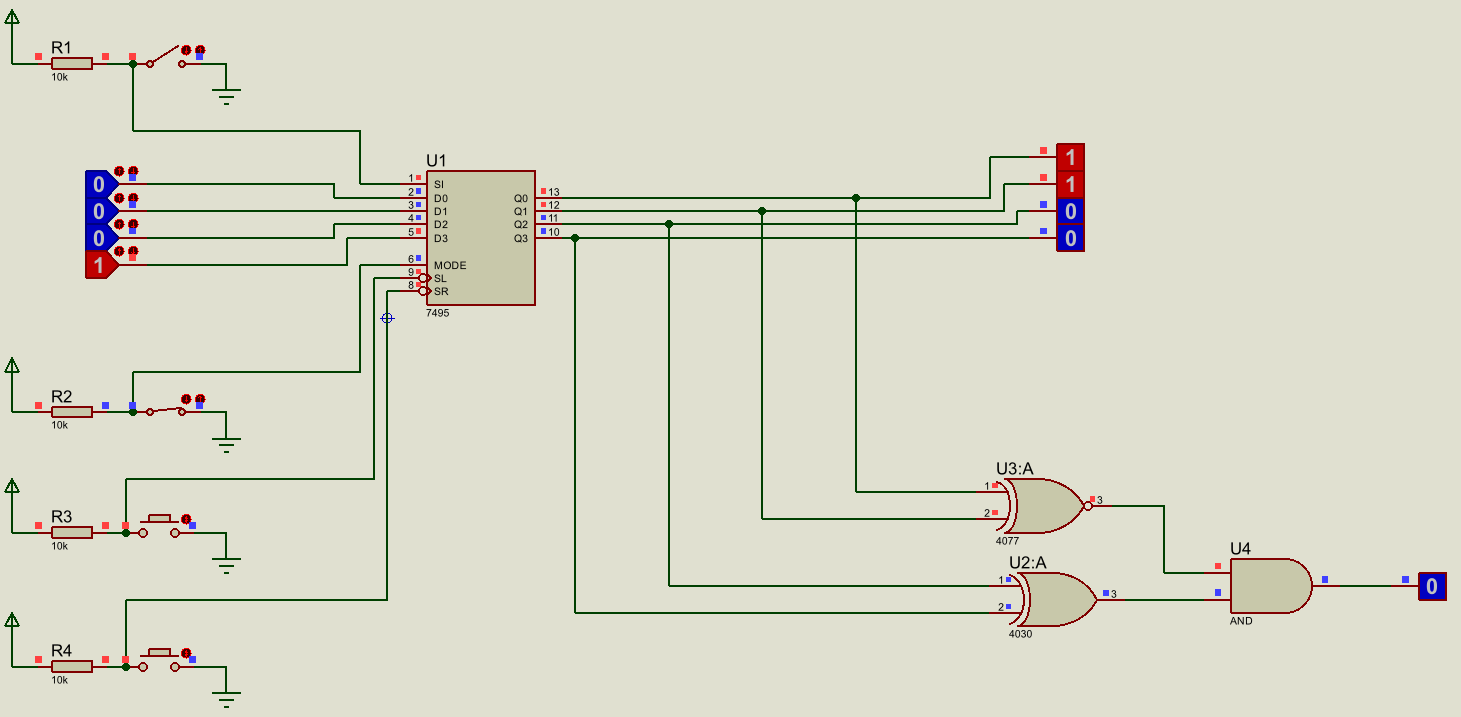
\includegraphics[width=1\textwidth]{images/2/t4.png}
    \captionof{figure}{یک شیفت راست با \lr{$S_{in} = 1$} نسبت به تصویر قبل}
    \label{fig:t4}
\end{center}


\section{نتیجه‌گیری}
	\leavevmode\par
	\vspace{0.3cm}

\begin{spacing}{1.3} 
در این آزمایش با طراحی داخلی شیفت‌رجیسترها آشنا شدیم و یک شیفت‌رجیستر را با استفاده از گیت‌های ساده و فلیپ‌فلاپ ها ساختیم. هم‌چنین با نحوه استفاده از ورودی کنترلی برای تغییر عملکرد شیفت‌رجیستر آشنا شدیم و شیفت‌رجیستری طراحی کردیم که بتواند بین کاربری‌های متفاوت، مانند شیفت به راست یا چپ، یا بارگذاری موازی و شیفت یک‌طرفه تغییر وضعیت دهد.

در ادامه از شیفت‌رجیستر آماده استفاده کردیم و با استفاده از تراشه 7495، مداری طراحی کردیم که بتواند رشته‌های چهاربیتی مدنظر را در ورودی تشخیص دهد.
\end{spacing}

\end{document}

